% !TEX root = ../thesis-example.tex
%
\chapter{Introduction}
\label{sec:intro}

%\cleanchapterquote{You can’t do better design with a computer, but you can speed up your work enormously.}{Wim Crouwel}{(Graphic designer and typographer)}

\blindtext \parencite{Duong2011}.

\begin{figure}
\caption{Here's a pretty picture.}
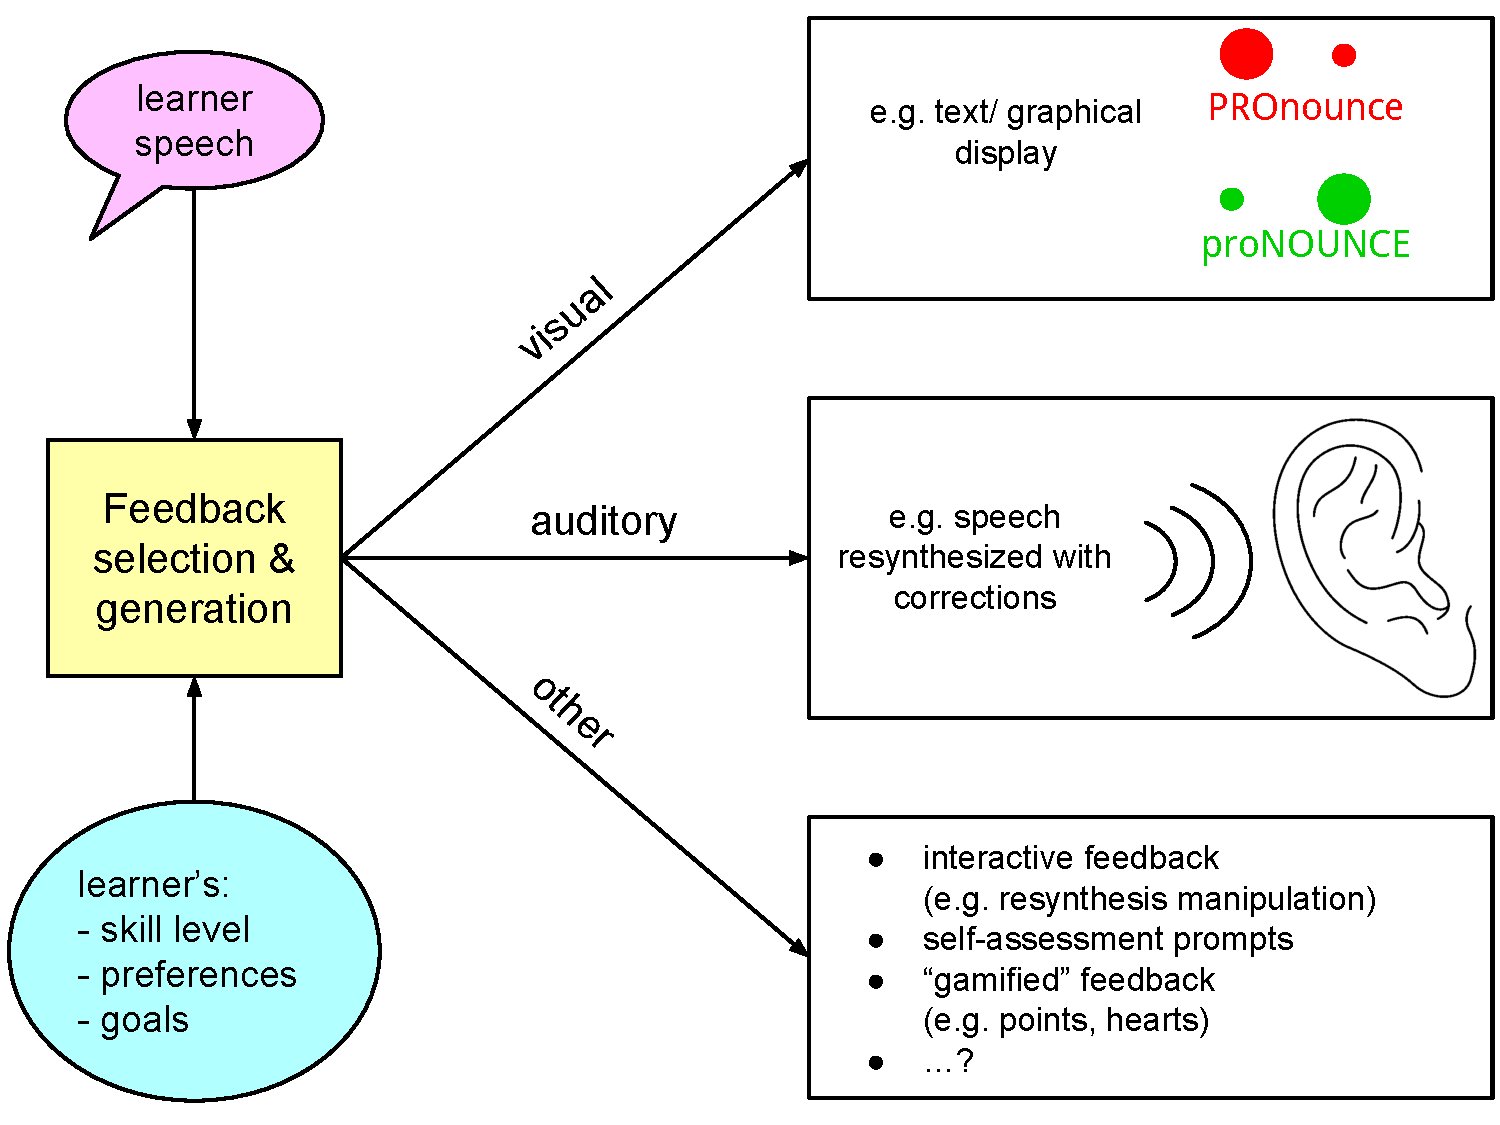
\includegraphics[width=.8\linewidth]{../img/feedback}
\end{figure}

\citeauthor{Sitaram2011} (\citeyear{Sitaram2011}) says blah blah blah.

\begin{table}
\caption{I made a table, isn't that awesome?}
\begin{tabular}{lll}
some & stuff & in \\
a & pretty & table \\
\end{tabular}
\end{table}


\section{Motivation and Problem Statement}
\label{sec:intro:motivation}

\Blindtext[3][1]

\section{Results}
\label{sec:intro:results}

\Blindtext[1][2]

\section{Thesis Structure}
\label{sec:intro:structure}

\textbf{Chapter \ref{sec:related}} \\[0.2em]
\blindtext

\textbf{Chapter \ref{sec:system}} \\[0.2em]
\blindtext

\textbf{Chapter \ref{sec:concepts}} \\[0.2em]
\blindtext

\textbf{Chapter \ref{sec:concepts}} \\[0.2em]
\blindtext

\textbf{Chapter \ref{sec:conclusion}} \\[0.2em]
\blindtext
